\documentclass{article}

% Language setting
% Replace `english' with e.g. `spanish' to change the document language
\usepackage[english]{babel}

% Set page size and margins
% Replace `letterpaper' with `a4paper' for UK/EU standard size
\usepackage[letterpaper,top=2cm,bottom=2cm,left=3cm,right=3cm,marginparwidth=1.75cm]{geometry}

% Useful packages
\usepackage{amsmath}
\usepackage{graphicx}
\usepackage[colorlinks=true, allcolors=blue]{hyperref}

\title{Logarithmic Potential in Lammps}
\author{Reyhaneh A. Farimani, \ Supervisor: Christos N. Likos}

\begin{document}
\maketitle

\begin{abstract}
In this report, I am going to implement a Logarithmic pair potential in the Lammps. 
\end{abstract}
\section{The pair potential:}
The pair potential needs three attributes:
\begin{itemize}
    \item cut-off($r_c$)
    \item particle Radius ($R$)
    \item constant energy multiplier for short distances($E_0$)
    \item constant energy multiplier for long distances($E_1$)
\end{itemize}
The Force and Energy Would be as follows:
\begin{equation}
    	U_{log/exp}(\lambda) =      
	\begin{cases}
		E_0 (-\ln x + 1/2e)
  & (r_{ij}\leq R)
  \\
    E_1e^{-bx^2}/2 
  & (R<r_{ij}\leq r_c)
  \\ 0 
  &
  r_{ij} > r_c
	\end{cases}
\end{equation}
\begin{equation}
    	F_{log/exp}(\lambda) =      
	\begin{cases}
		E_0 (-\frac{1}{x})
  & (r_{ij}\leq R)
  \\
		E_1 b (-x e^{-x^2})
  & (R<r_{ij}\leq r_c)
  \\ 0 
  &
  r_{ij} > r_c
	\end{cases}
\end{equation}
In which $x = \frac{r_{ij}}{R}$.
We would like the potential and its derivative (force), to be continuous, so we are going to define $E_1$ and $b$ based on the following:
\[
E_1 e^{-b} / 2 = E_0 (-\ln(1) + \frac{1}{2e})  = E_0 \frac{1}{2e}
\]
\[
 b E_1 e^{-b} = E_0
\]
\begin{equation}
    \Rightarrow b = e,\quad E_1 = E_0 e^{e-1} 
\end{equation}
So, we update the old equations with new parameters:
\begin{equation}
    	U_{log/exp}(\lambda) =      
	\begin{cases}
		E_0 (-\ln x + 1/2e)
  & (r_{ij}\leq R)
  \\
    E_0 e^{-ex^2 +e -1}/2 
  & (R<r_{ij}\leq r_c)
  \\ 0 
  &
  r_{ij} > r_c
	\end{cases}
\end{equation}
\begin{equation}
    	F_{log/exp}(\lambda) =      
	\begin{cases}
		E_0 (-\frac{1}{x})
  & (r_{ij}\leq R)
  \\
		E_0 (-x e^{-ex^2 + e})
  & (R<r_{ij}\leq r_c)
  \\ 0 
  &
  r_{ij} > r_c
	\end{cases}
\end{equation}
We have developed, and for the two bodies, it was tested, and shown in figure \ref{fig:test:1}, \ref{fig:test:2}.
\begin{figure}
    \centering
    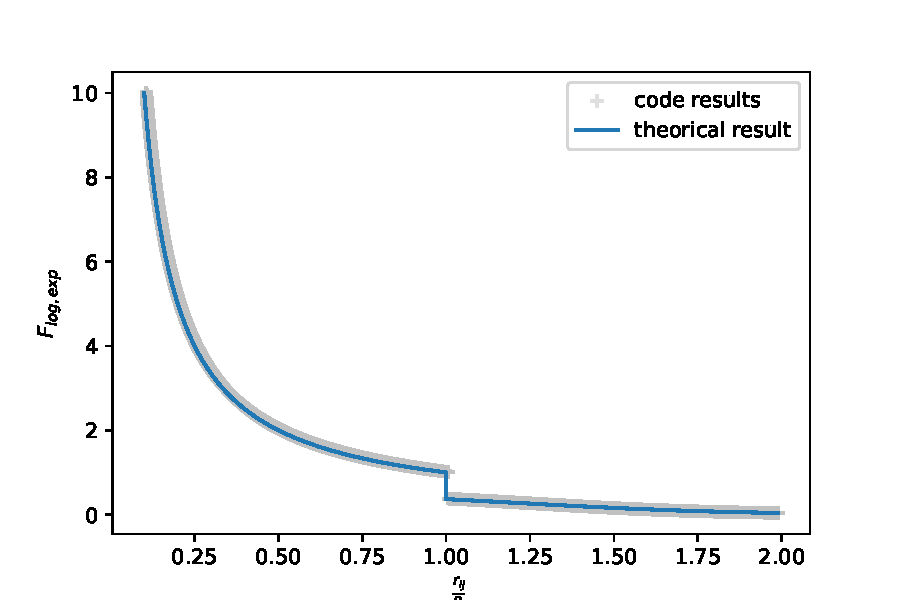
\includegraphics{test_2_body.pdf}
    \caption{two body tests of pair potential (Force)}
    \label{fig:test:1}
\end{figure}
\begin{figure}
    \centering
    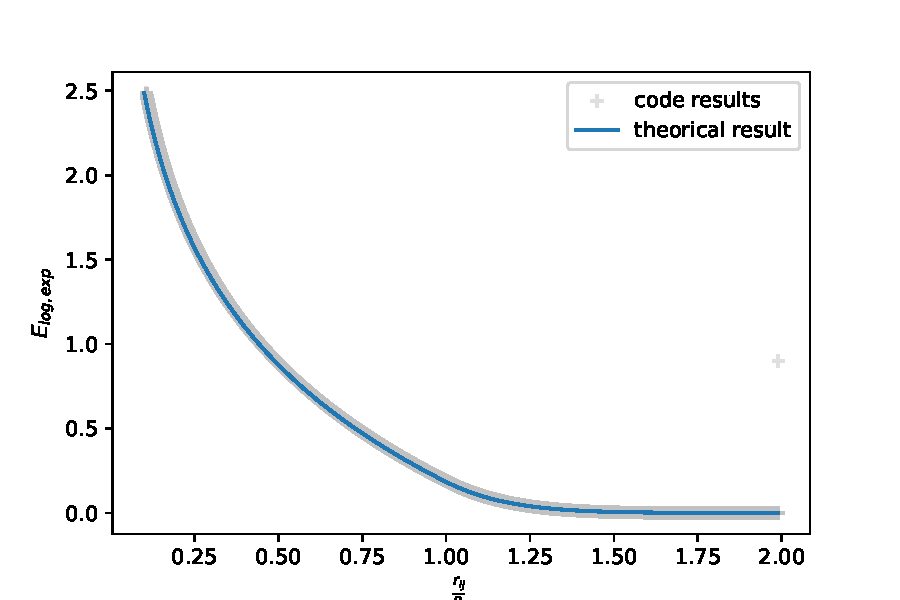
\includegraphics{test_2_body_energy.pdf}
    \caption{two body tests of pair potential (Energy)}
    \label{fig:test:2}
\end{figure}
There is some inaccuracy in the potential results. Currently, I am fixing it. (Update on 8Sep Afternoon: fixed)
\\
The next step is to check for many-body systems (Update on 8Sep Afternoon: tested), and then we go through two-dimensional many-body systems for the thesis work.
\end{document}